% This is "sig-alternate.tex" V2.0 May 2012
% This file should be compiled with V2.5 of "sig-alternate.cls" May 2012
%
% This example file demonstrates the use of the 'sig-alternate.cls'
% V2.5 LaTeX2e document class file. It is for those submitting
% articles to ACM Conference Proceedings WHO DO NOT WISH TO
% STRICTLY ADHERE TO THE SIGS (PUBS-BOARD-ENDORSED) STYLE.
% The 'sig-alternate.cls' file will produce a similar-looking,
% albeit, 'tighter' paper resulting in, invariably, fewer pages.
%
% ----------------------------------------------------------------------------------------------------------------
% This .tex file (and associated .cls V2.5) produces:
%       1) The Permission Statement
%       2) The Conference (location) Info information
%       3) The Copyright Line with ACM data
%       4) NO page numbers
%
% as against the acm_proc_article-sp.cls file which
% DOES NOT produce 1) thru' 3) above.
%
% Using 'sig-alternate.cls' you have control, however, from within
% the source .tex file, over both the CopyrightYear
% (defaulted to 200X) and the ACM Copyright Data
% (defaulted to X-XXXXX-XX-X/XX/XX).
% e.g.
% \CopyrightYear{2007} will cause 2007 to appear in the copyright line.
% \crdata{0-12345-67-8/90/12} will cause 0-12345-67-8/90/12 to appear in the copyright line.
%
% ---------------------------------------------------------------------------------------------------------------
% This .tex source is an example which *does* use
% the .bib file (from which the .bbl file % is produced).
% REMEMBER HOWEVER: After having produced the .bbl file,
% and prior to final submission, you *NEED* to 'insert'
% your .bbl file into your source .tex file so as to provide
% ONE 'self-contained' source file.
%
% ================= IF YOU HAVE QUESTIONS =======================
% Questions regarding the SIGS styles, SIGS policies and
% procedures, Conferences etc. should be sent to
% Adrienne Griscti (griscti@acm.org)
%
% Technical questions _only_ to
% Gerald Murray (murray@hq.acm.org)
% ===============================================================
%
% For tracking purposes - this is V2.0 - May 2012

\documentclass{acm_proc_article-sp}

\usepackage{graphicx}
\usepackage{caption}
\usepackage{subcaption}
\usepackage{url}
\usepackage{subfigure}
\usepackage{tikz}
\usetikzlibrary{arrows,positioning} 

% Redefines \@ptsize to make setspace happy
% \makeatletter
% \renewcommand{\@ptsize}{0}
% \makeatother

% Double-spaces the entire document
%\usepackage{setspace}
%\doublespacing

\begin{document}
%
% --- Author Metadata here ---
\conferenceinfo{ICMI}{'13 Sydney Australia}
%\CopyrightYear{2007} % Allows default copyright year (20XX) to be over-ridden - IF NEED BE.
%\crdata{0-12345-67-8/90/01}  % Allows default copyright data (0-89791-88-6/97/05) to be over-ridden - IF NEED BE.
% --- End of Author Metadata ---

\title{ChAirGest 2013 - Temporal Segmentation Optimization for Continuous Gesture 
Recognition}
%
% You need the command \numberofauthors to handle the 'placement
% and alignment' of the authors beneath the title.
%
% For aesthetic reasons, we recommend 'three authors at a time'
% i.e. three 'name/affiliation blocks' be placed beneath the title.
%
% NOTE: You are NOT restricted in how many 'rows' of
% "name/affiliations" may appear. We just ask that you restrict
% the number of 'columns' to three.
%
% Because of the available 'opening page real-estate'
% we ask you to refrain from putting more than six authors
% (two rows with three columns) beneath the article title.
% More than six makes the first-page appear very cluttered indeed.
%
% Use the \alignauthor commands to handle the names
% and affiliations for an 'aesthetic maximum' of six authors.
% Add names, affiliations, addresses for
% the seventh etc. author(s) as the argument for the
% \additionalauthors command.
% These 'additional authors' will be output/set for you
% without further effort on your part as the last section in
% the body of your article BEFORE References or any Appendices.

\numberofauthors{2} %  in this sample file, there are a *total*
% of EIGHT authors. SIX appear on the 'first-page' (for formatting
% reasons) and the remaining two appear in the \additionalauthors section.
%
\author{
% You can go ahead and credit any number of authors here,
% e.g. one 'row of three' or two rows (consisting of one row of three
% and a second row of one, two or three).
%
% The command \alignauthor (no curly braces needed) should
% precede each author name, affiliation/snail-mail address and
% e-mail address. Additionally, tag each line of
% affiliation/address with \affaddr, and tag the
% e-mail address with \email.
%
% 1st. author
\alignauthor
Ying Yin\\
       \affaddr{Massachusetts Institute of Technology}\\
       \affaddr{}\\
       \affaddr{}\\
       \email{yingyin@csail.mit.edu}
% 2nd. author
\alignauthor
Randall Davis \\
       \affaddr{Massachusetts Institute of Technology}\\
       \affaddr{}\\
       \affaddr{}\\
       \email{davis@csail.mit.edu}
}

\maketitle
\begin{abstract}
We propose a novel approach of accurately detecting the start of a gesture nucleus phase.
\end{abstract}

%A category including the fourth, optional field follows...
\category{H.5.2}{Information Systems}{Information Interfaces and
Presentation}[User Interfaces]

\keywords{Continuous gesture recognition, temporal segmentation, HMM}

\section{Introduction}

\section{System Overview}
We use both Kinect and Xsens data to extract hand motion feature vector $X_t$ for gesture modeling. 
It is relatively easy to obtain features from the Xsens data. We choose to use linear
acceleration (x, y, z), angular velocity (x, y, z) and Euler orientation (yaw, pitch, roll)
from the Xsens unit on the hand to form a 9-dimensional feature vector, $X_{\text{xsens}}$.

\begin{figure*}
\centering
\includegraphics[width=1\linewidth]{fig/system.ps}
\caption{System overview of our gesture recognition framework. }
\label{fig:system}
\end{figure*}

Feature extraction on video sequences is often done in two steps: 1)
detect points of interest by maximizing certain salience functions; 2) compute
feature descriptors to capture shape and motion in the neighborhoods of the selected
points~\cite{wang-spatio-2009}.

For hand gesture recognition, the points of interest are certainly the hands. While the skeleton tracking provided
by the Kinect SDK is quite robust most of the time, its error for hand joint tracking increases when
the hands are close to the body or move quickly (see Figure~\ref{fig:compare-skeleton}). As a result, we
developed a gesture salience detection method to locate the gesturing hand more accurately.

The final stream of feature vectors are input to the HMM-based
gesture recognition framework for classification. Figure~\ref{fig:system} shows the overview of the entire process.
The following sections give detailed explanation of our method.  

\section{Gesture Salience Detection}
Similar to Marcos-Ramiro et al.~\cite{marcos2013}, we define gesture salience as a function of 
the closeness of the motion to the observer (e.g., the camera) and the magnitude of the motion,
and compute it from both the RGB and the depth data. Both the RGB and the depth data can be noisy. RGB cameras are sensitive to lighting conditions.
Skin color based detection can be sensitive to the clothes users wear. Depth cameras based on 
structured light sensors, such as the first generation Kinect sensor, compare the projected infra-red pattern
with the reflected one to determine depth~\cite{welsh:2011}. As a result, they do not work well on 
objects that are highly reflective (mirrors and shiny metal) or highly absorptive (fluffy and/or dark materials such as human hair)
\footnote{\url{http://msdn.microsoft.com/en-us/library/hh855356.aspx}}. By combining both RGB and
depth information
the overall gesture salience detection can be more robust.

The following are the detailed steps of our gesture salience detection method for each frame. 
We show the illustrations in Figure~\ref{fig:gesture-salience}. 

\subsection{Skin Segmentation}
To make our method generalizable to any users and environment, we use an off-the-shelf simple skin color detection method which is not trained on our data set to do a binary segmentation. 
. We compute a binary skin mask, $M^S$, based on the RGB image converted into YCrCb
color space.  We also find the user mask, $M^U$ obtained from the Kinect SDK based on the depth image. 
We then align $M^S$ with $M^U$ and find their intersection $M^{S\wedge U}$, which indicates the skin region on the user.

\subsection{Motion Detection}
Similar to Cutler and Turk~\cite{cutler1998}, we compute the motion mask for the current depth frame based on 3 frames. We first filter each 
depth frame by the user and skin mask $M^{S\wedge U}$ at time $t$, and then
smooth it through a median filter to obtain $D_t$, which is basically a depth image containing user's skin region only (see Figure~\ref{fig:skin-mask}).
Equation~(\ref{eq:motion-mask}) computes the binary mask, $M_{t\vee t-1}^M$, indicating pixels whose depth values have changed from time $t-1$ to $t$ (Figure~\ref{fig:motion-mask}).
$D_{t\vee t-1}^{D}$ is the absolute difference between $D_t$ and $D_{t-1}$, and $T$ is the threshold operator that filters out small change in depth value 
(we set the threshold to be 15mm). 
To obtain the motion mask, $M_{t}^M$ for time $t$ only, we use $M_{t-1\vee t-2}^M$, the motion mask for $t-1$ and $t-2$ as well (see Equation~(\ref{eq:motion-mask-t-1})-(\ref{eq:motion-mask-t}),
 AND and XOR indicated by $\wedge$ and $\oplus$).
\begin{align}
M_{t\vee t-1}^M &= T(D_{t\vee t-1}^{D}) \label{eq:motion-mask} \\
M_{t-1}^M &= M_{t\vee t-1}^M \wedge M_{t-1\vee t-2}^M \label{eq:motion-mask-t-1}\\
M_{t}^M &= M_{t\vee t-1}^M \oplus M_{t-1}^M \label{eq:motion-mask-t}
\end{align}

\subsection{Salience Map}
We compute histograms of depth values in both $D_t$ and $D_{t\vee t-1}^{D}$ and then apply histogram normalization to obtain cumulative distributions $H_t$ and $H_{t\vee t-1}^D$.
$H_t$ represents the probability of salience given a depth value, while $H_{t\vee t-1}^D$ represents the probability of salience given
a depth difference value. The lower the depth value or the higher the depth difference value, the higher the salience probability. The reason for using
histogram equalization is to reduce the effect of outliers such that a single large depth value will not suppress the salience probabilities of other depth values. 
Finally the salience map (Figure~\ref{fig:salience}) can be computed for each pixel $(x, y)$ as
\begin{align}
S_t(x, y) = H_t(D_t(x, y)) \times H_{t\vee t-1}^D(D_t^D(x, y)) \times M_t^M
\end{align}
The multiplication of the binary motion mask $M_t^M$ allows us to consider only the motion due to the user at $t$.
 
\subsection{Salience Location}
The final step of locating the most salient region in a frame is finding the
contour, $C_t$, from the salience map $S_t$ that has a perimeter greater than
the smallest possible hand perimeter and with the highest average salience for all the pixels inside the contour.

When motion is slow, the motion mask usually indicates the edge of the moving
object. As a result, the center of $C_t$ may not be the center of the moving
object (in our case, the user's hand). Hence, we use 2 iterations of Camshift~\cite{Bradski98} on the depth image $D_t$ with a start search location at the center of $C_t$ to refine
the final bounding box, $B_t$, of gesture salience (Figure~\ref{fig:camshift}).

\begin{figure*}[tb]
\centering
\hspace{-0.6em}%
\subfigure[]{
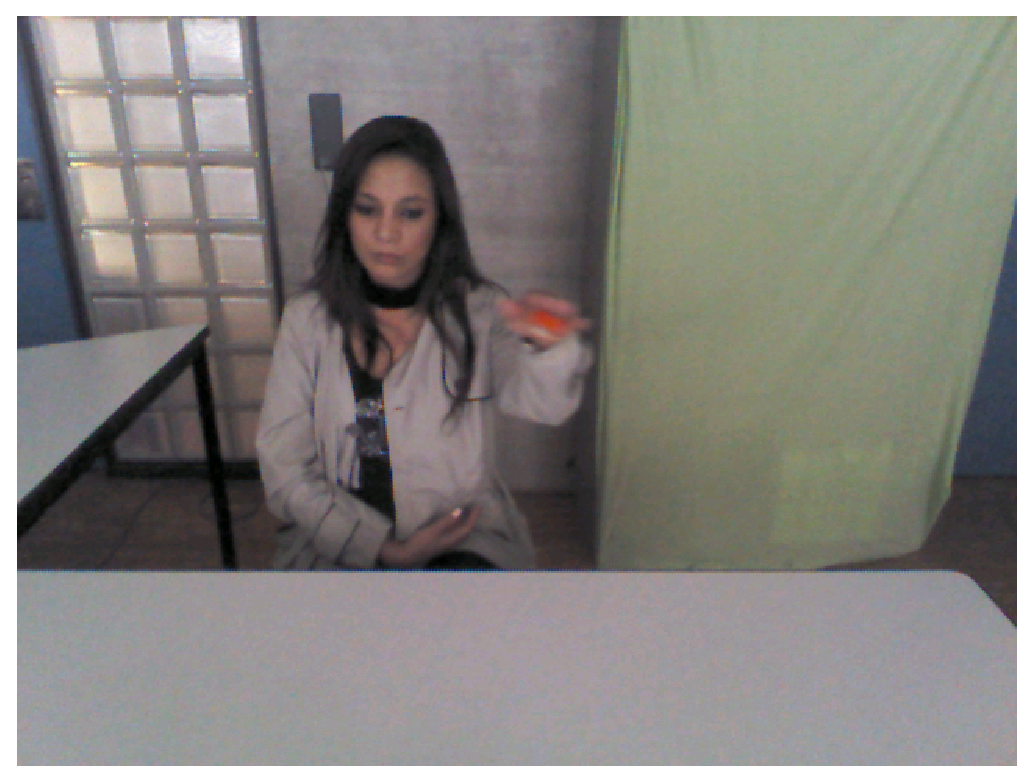
\includegraphics[width=0.19\linewidth]{figure/color.eps}\hspace{-0.6em}%
\label{fig:color}
}
\subfigure[]{
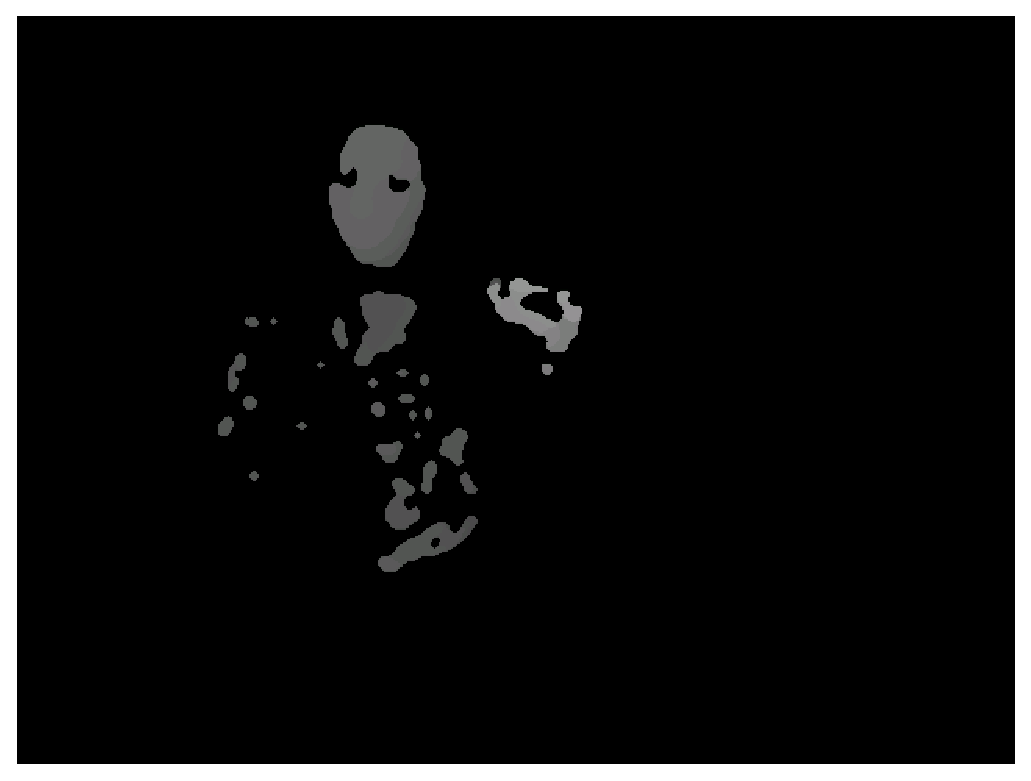
\includegraphics[width=0.19\linewidth]{figure/depth.eps}\hspace{-0.6em}
\label{fig:skin-mask}
}
\subfigure[]{
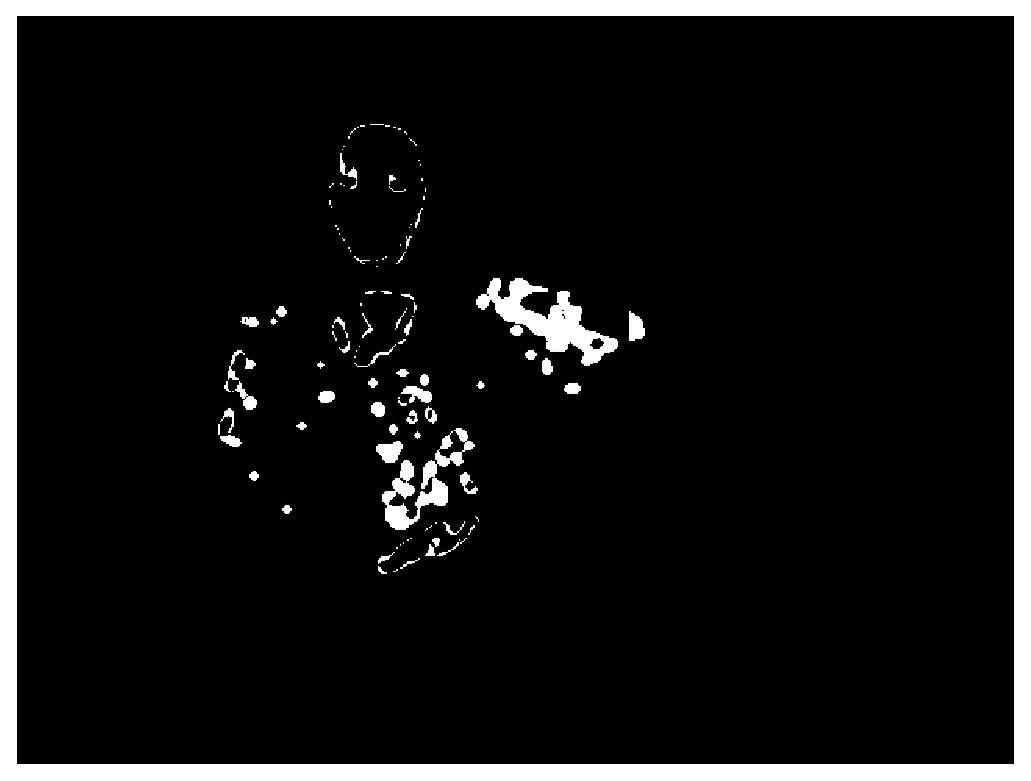
\includegraphics[width=0.19\linewidth]{figure/motion-mask1.eps}\hspace{-0.6em}
\label{fig:motion-mask}
}
\subfigure[]{
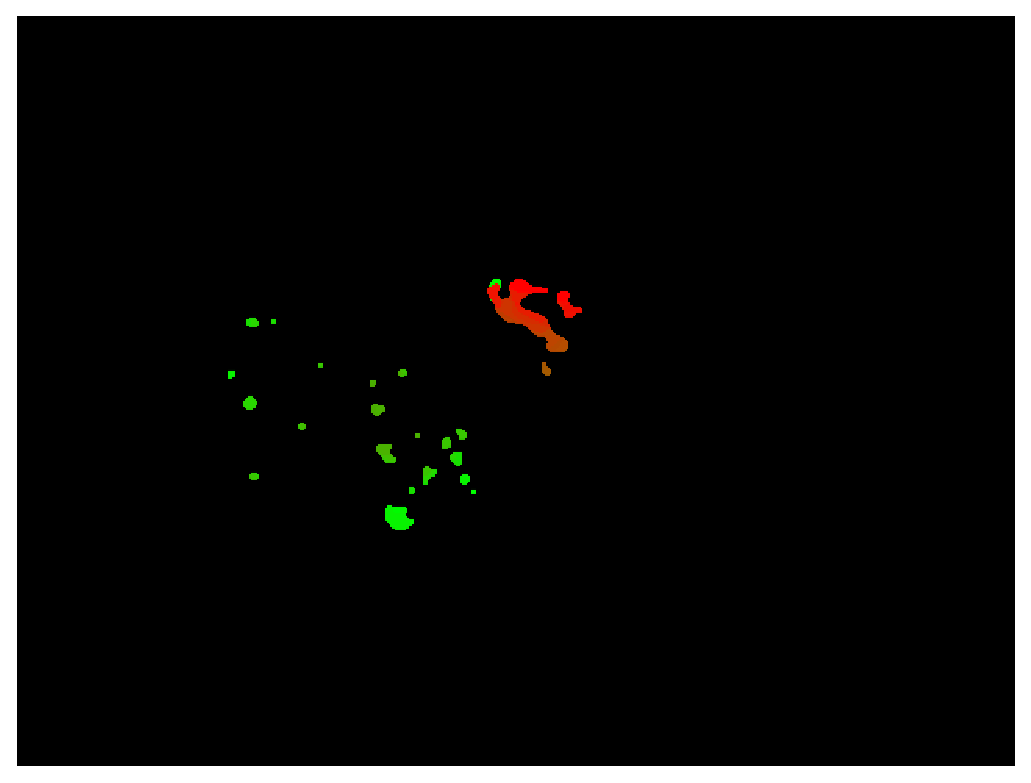
\includegraphics[width=0.19\linewidth]{figure/salient-map.eps}\hspace{-0.6em}
\label{fig:salience}
}
\subfigure[]{
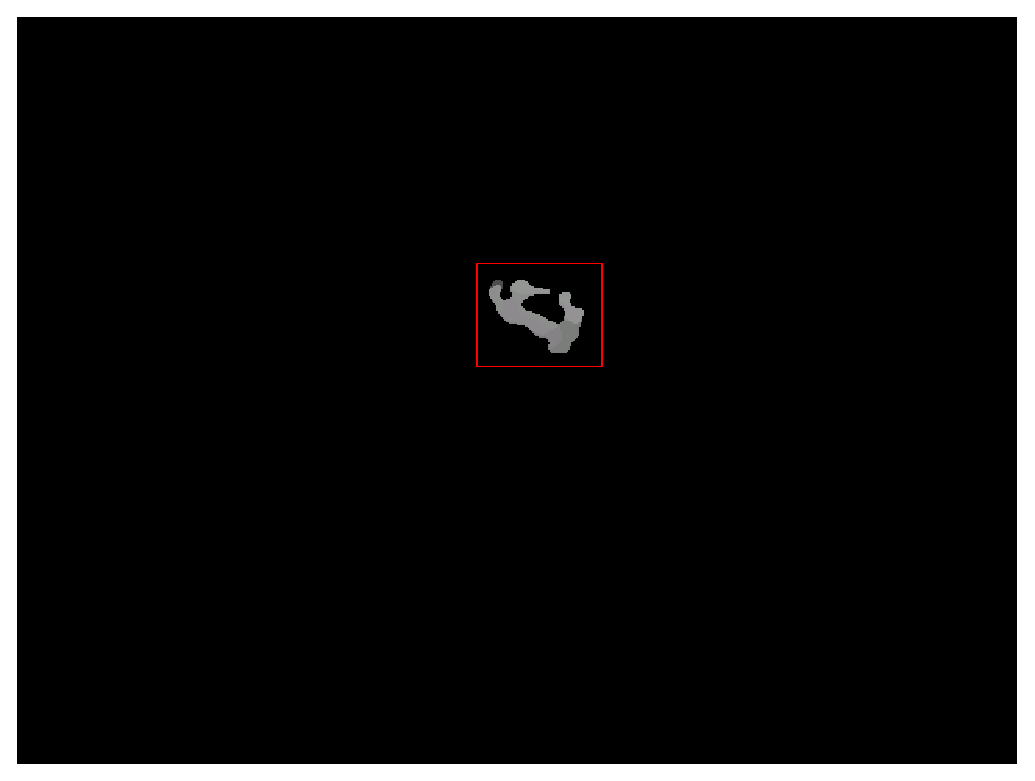
\includegraphics[width=0.19\linewidth]{figure/bounding-box.eps}
\label{fig:camshift}
}
\caption{Gesture salience detection steps: \subref{fig:color} RGB image under low lighting condition;
\subref{fig:skin-mask} depth map $D_t$ filtered by skin and user mask, $M^{S\wedge U}$. False detection of skin due to
clothes color similar to skin color; \subref{fig:motion-mask} motion mask,  $M_{t\vee t-1}^M$, indicating moved pixels for time $t$ and $t-1$;
\subref{fig:salience} salience map with red color indicating high probability of the salience; 
\subref{fig:camshift} final gesture salience bounding box, $B$. (Best viewed in
color.)}
\label{fig:gesture-salience}
\end{figure*}

Figure~\ref{fig:compare-skeleton} compares the results of gesture salience detection for hand gestures with the skeleton tracking results
from the Kinect SDK.
\begin{figure*}
\centering
\subfigure[]{
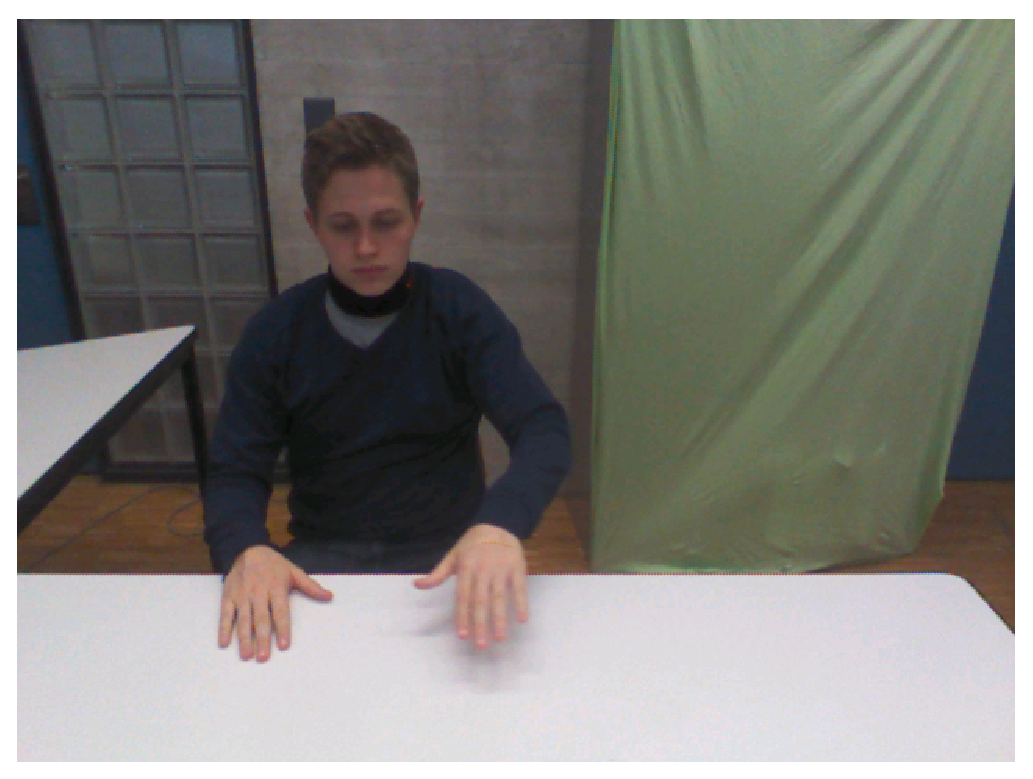
\includegraphics[width=0.23\linewidth]{fig/rotate-color.eps} \hspace{-0.6em}
}
\subfigure[]{
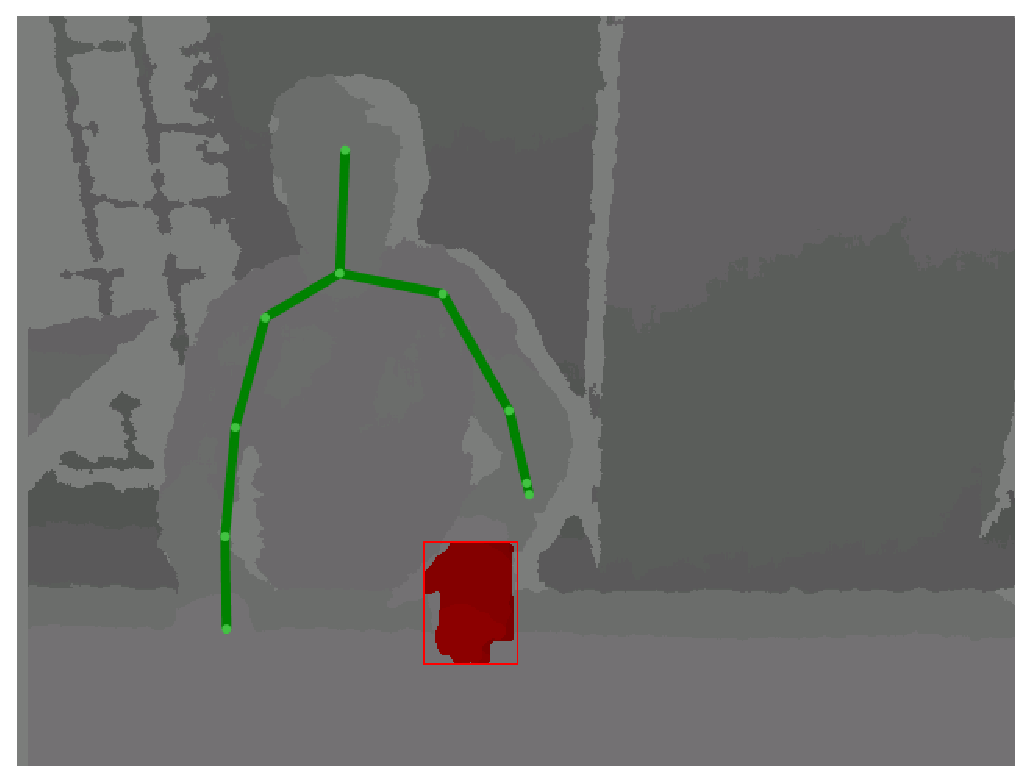
\includegraphics[width=0.23\linewidth]{fig/rotate-depth.eps} \hspace{-0.6em}
}
\subfigure[]{
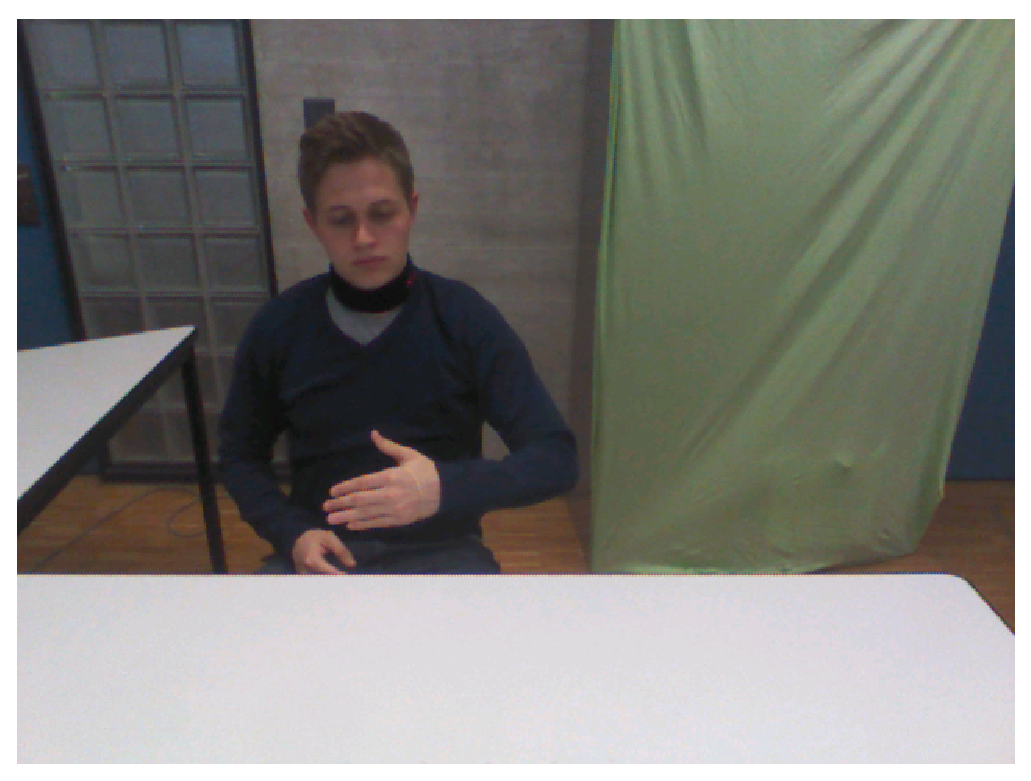
\includegraphics[width=0.23\linewidth]{fig/near-body-color.eps}
\hspace{-0.6em} }
\subfigure[]{
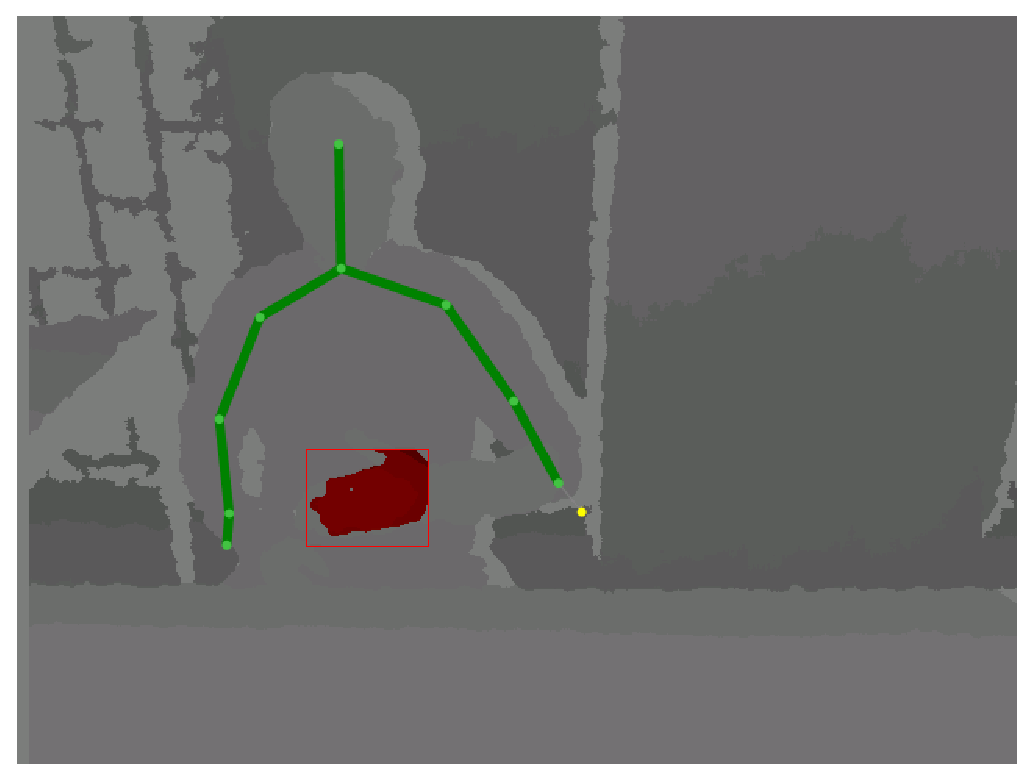
\includegraphics[width=0.23\linewidth]{fig/near-body-depth.eps}
\hspace{-0.6em} }
\caption{Comparison between gesture salience detection for hand gestures and skeleton tracking from the Kinect SDK. The green lines are
the skeleton tracking results. The red region is the detected salient gesture
region using our method. (Best viewed in color.)}
\label{fig:compare-skeleton}
\end{figure*}

\subsection{Hand Feature}
We combine the relative hand positions from the gesture salience detection and the other hand 
motion features from the Xsens to form the final feature vector. both hand motion features, $X^M_t$ and hand pose features, $X^P_t$
for the observed feature vector $X_t$, i.e., 
\begin{displaymath}
X_t = \left[ \begin{array}{c}
X^M_t\\
X^P_t
\end{array}\right]
\end{displaymath} 

The motion features include the relative position ($\bf{p}$), velocity ($\bf{v}$),
and acceleration ($\bf{a}$) of the center of
the hand bounding box.
All of them are 3-dimensional vectors in the world
coordinate system, hence $X_t^M\in\mathbb{R}^9$. 

The hand pose features are computed from a $100 \times 100$ px image $I_{h}$ scaled
from the bounding box of the final tracked hand (Figure~\ref{fig:depth}). Each pixel
is a depth value scaled between $0$ and $255$. We explore several hand pose 
features derived from $I_h$.

\section{Temporal Segmentation of Continuous Gestures}\label{sec:recognition}
\subsection{Rest Position Modeling}
We use all the training data from all users to create a Gaussian model for the rest 
positions and a Gaussian model for non-rest positions.

During recognition, an observation $X_t$ at time frame $t$ is first classified into 
rest or non-rest position. It is non-rest position if 
\begin{displaymath}
N(X_t; \mu_{\text{NON-REST}}, \Sigma_{\text{NON-REST}}) \geq N(X_t; \mu_{\text{REST}}, \Sigma_{\text{REST}})
\end{displaymath}
Where $N$ represents the Gaussian probability. Sequences of continuous observations from non-rest
positions longer than 0.25s are further classified into different gestures based on the trained HMM model.
 
\subsection{Temporal Gesture Modeling and Training}
Previous research suggests that
a gesture consists three phases: pre-stroke (also called preparation), nucleus, and post-stroke 
(also called retraction)~\cite{Pavlovic97}. The preparation phase consists
of a preparatory movement that sets the hand in motion from some resting position.
The nucleus of a gesture has some ``definite form and enhanced dynamic qualities''
~\cite{kendon86}. Finally, the hand either returns to the resting position or repositions
for the new gesture phase. Each gesture has a unique nucleus phase, but gestures can
share similar preparation and retract phases~\cite{krahnstoever2002}. Each gesture
phase includes a sequence of hand/arm movement which can be modeled using HMMs. 

Because we have the ground truth labeling of the pre-stroke, nucleus and post-stroke phases, 
we can train an HMM for each phase for each gesture. 

As each phase can have variable length, we model the termination probability for each
hidden state $s$ as $t(\text{END}|s)$. Given a sequence of observation $\underline{X}_1^T = \underline{x}_1\ldots\underline{x}_T$, and 
the corresponding hidden states sequence $S_1^T = s_1\ldots s_T$, we difine the probability
\begin{displaymath}
p(\underline{X}_1^T, S_1^T;\underline{\theta}) = 
    t(s_1)t(END|s_T)\prod_{t = 2}^T t(s_t | s_{t-1})\prod_{t = 1}^T e(\underline{x}_t|s_t)
\end{displaymath}
where $\underline{\theta}$ represents the model parameter vector which includes
the initial state probabilities $t(s)$, the state transition probabilities $t(s'|s)$, and the 
emission probabilities $e(\underline{x}|s)$ for $s, s'\in \{1, 2,\ldots k\}$. 

We use a mixture of Gaussians for the emission probability to model user variations, i.e.
\begin{displaymath}
e(\underline{x}_t|s_t) = \sum_{q_t = 1}^l g(q_t | s_t)N(x_t; \mu_{s_t,q_t}, \Sigma_{s_t,q_t})
\end{displaymath} 

Given $N$ training sequences, We use the Expectation Maximization (EM) algorithm to estimate the model parameters. In
particular, the update for the termination probability during the $i$th iteration is 
\begin{displaymath}
t^i(END|s) = \frac{\sum_{j = 1}^N \overline{count}(j, s\rightarrow END;\underline{\theta}^{i-1})}
    {\sum_{j = 1}^N\sum_{s'} \overline{count}(j, s\rightarrow s';\underline{\theta}^{i-1})}
\end{displaymath}
where $\overline{count}(j, s\rightarrow END;\underline{\theta}^{i-1})$ is the expected count of 
$s$ being the end state. We can use the usual forward-backward algorithm to compute all the 
expected sufficient statistics by adding a dummy END state to the end of each sequence.

Because there are 3 rest positions, we use 3 hidden states for both the pre-stroke and post-stroke phases.
Each hidden state can be the start state and can only remain in its own state or go to the end state.
 
For the nucleus phase, we use a modified Bakis~\cite{} model to constrain the transition probabilities
among the hidden states. Instead of only allowing left-right transition, we allow the last hidden state
to go back to the initial state. This is particularly important for modeling gestures with arbitrary number of
repetitions such as waving and shaking hands. 

\tikzstyle{vertex}=[circle, draw, minimum size=16pt, inner sep=0pt]
\tikzstyle{observed-vertex}=[circle, draw, minimum size=16pt, inner
sep=0pt, fill=black!20] 
\tikzstyle{edge} = [draw, thick, -]
\tikzstyle{directed-edge} = [draw, ->]

\begin{figure}[tb]
\centering
  \begin{tikzpicture}[auto,swap, scale=1.5]
    % First we draw the vertices
    \foreach \pos/\name in {{(0, 0)/start}, {(1, 0)/s_1}, {(2, 0)/s_2},
    {(3, 0)/s_3}, {(4, 0)/s_4}, {(5, 0)/end}}
      \node[vertex] (\name) at \pos {$\name$};
    % Connect vertices with edges and draw weights
    \foreach \source/ \dest in {s_2/s_3, s_3/s_4, s_4/end,
    s_1/s_2} \path[directed-edge] (\source) -- (\dest);
    
    \foreach \source/ \dest in {s_1/s_3, start/s_2, s_2/s_4, s_3/end, s_4/s_1} 
      \path[directed-edge] (\source) edge [bend left] (\dest);
      
    \foreach \source/ \dest in {s_1/s_1, s_2/s_2, s_3/s_3, s_4/s_4} 
      \path[directed-edge] (\source) edge [loop above] (\dest);
    
    \path[directed-edge] (start) edge node [below] {$t(s_1)$} (s_1);
  \end{tikzpicture}
  \caption{The state transition diagram of a modified four-state Bakis model.}
  \label{fig:bakis}
\end{figure}

\subsection{Gesture Recognition}
During the recognition phase, we concatenate the HMMs trained for each phase together to form
one HMM for every gesture. The transition probability from the previous phase to the next
phase can be computed by multiplying the termination probabilities of the previous phase and the
initial state probabilities of the next phase. Using the superscript $c$ to denote the model
parameters in the concatenated HMM, we have
\begin{displaymath}
t^c(s_\text{nucleus}|s_\text{prestroke}) = t(\text{END}|s_\text{prestroke}) \times t(s_\text{nucleus})
\end{displaymath}

As new state transition probabilities are added, the transition probabilities among
states in the same phase also need to be modified so that $\sum_{s' = 1}^K t(s'|s) = 1$ (where
$K$ is the total number of combined hidden states) is ensured. For example
\begin{displaymath}
t^c(s'_{\text{nucleus}} | s_{\text{nucleus}}) = t(s'_{\text{nucleus}} | s_{\text{nucleus}})
  \times (1 - t(\text{END} | s_{\text{nucleus}}))
\end{displaymath}

We also add a rest state to the end of the HMM and allow the rest state to transit to pre-stroke
and post-stroke phase with uniform probabilities to accommodate short pauses during the gesture.
Let $\underline{\theta}_g$ be the final concatenated HMM for gesture $g$. The classification
for an observation sequence from non-rest positions is:
\begin{displaymath}
\hat{g} = \arg\max_g\log p(\underline{X}_1^T; \underline{\theta}_g)
\end{displaymath}

\subsection{Identify the Start of Nucleus Phase}
Because the non-rest positions include both pre-stroke and post-stroke phases, we need
to identify the start of the actual gesture (nucleus). We use the Viterbi algorithm
to find the most probable hidden state sequence $\hat{s}_1\ldots\hat{s}_T$ for a given observed sequence using 
the mostly likely gesture model $\underline{\theta}_{\hat{g}}$. The start and end time for the gesture nucleus is
the first and the last time frames $t$ where $\hat{s}_t\in s_{\text{nucleus}}$. Note that
we are able to identify whether a hidden state belongs to the nucleus phase because we trained the three phases
separately.

\section{Experimental Evaluation}\label{sec:eval}
We present our evaluation result based on the development data set of the ChAirGest corpus~\cite{Ruffieux2013}.

\subsection{Method}
For each participant, we use
one tenth of the sequences for testing and the remaining for training. The RGB and depth videos are 30 fps (frame per second) and we down-sample them
to 10 fps to increase the training speed. This results in about 600 frames per sequence on average.

\subsection{Hand Pose Feature Comparison}
Table~\ref{tab:comp-feature} shows the comparison of the recognition performance with different hand pose features $X_t^P$. The 
hand motion feature $X_t^M$ is kept the same. All results are based on fixed-interval smoothing inference.
Note that $n$ is the number of PCA components mentioned in Section~\ref{sec:eigenhand} and $sBin$ is the
cell size and $oBin$ is the number of orientation bins mentioned in Section~\ref{sec:hog}.

\begin{table}[tb]
\begin{center}
\caption{Per frame gesture classification accuracy and F1 scores in \% for different
hand pose features on the test data set. The results are the average from all test
sequences from 4 participants. Numbers in parentheses are standard deviations.}
\label{tab:comp-feature}
\begin{tabular}{|l|c|c|}
\hline
\textbf{Hand pose feature} & \textbf{Accuracy} & \textbf{F1} \\
\hline
Eigenhand (d = 7) & 83.3 (4) & 74.8 (8) \\ 
\hline
HOG (sBin = 4, oBin = 9, d = 7) & 84.0 (3) & 79.7 (8)\\
\hline
HOG (sBin = 8, oBin = 9, d = 7) & 84.0 (3) & 74.6 (2)\\
\hline
HOG (sBin = 30, oBin = 12, d = 7) & 70.9 (6) & 70.9 (9)\\
\hline
\end{tabular}
\end{center}
\end{table}

\subsection{Gesture classification confusion matrix}
Using fixed-interval smoothing inference and the same hand pose feature in the previous
section, we compute the frame-based confusion matrix
between the ground truth gesture labels and the predicted ones. Figure~\ref{fig:confusion-matrix} shows that most gesture phase classification errors
occur between the preparation (\#11) phase / the retraction (\#12) phase and the other gesture nucleus phases. We
observe that the transitions between these phases are usually
not very clear even to the human eyes, and hence accurate detection of the boundaries between these
phases can be hard. For many applications, the accurate detection of the boundaries may not be
necessary either.

We also note that this data set has a few gestures that are particularly hard to recognize.
For example the ``Palm-up rotation'' gesture (\#10) is similar to the ``Swipe right'' gesture (\#3) as they 
have the same motion trajectory. The difference is that the hand rotates in the ``Palm-up rotation'' gesture whereas the 
hand stays the same in the ``Swipe right'' gesture. However, some participants rotate their hands when doing
the ``Swipe right'' gesture as well (see Figure~\ref{fig:swipe-right}).

\section{Conclusions}
 
%\end{document}  % This is where a 'short' article might terminate

% The following two commands are all you need in the
% initial runs of your .tex file to
% produce the bibliography for the citations in your paper.
\bibliographystyle{abbrv}
\bibliography{sigproc}  % sigproc.bib is the name of the Bibliography in this case
% You must have a proper ".bib" file
%  and remember to run:
% latex bibtex latex latex
% to resolve all references
%

\balancecolumns % GM June 2007
% That's all folks!
\end{document}
